\documentclass[sigconf]{acmart}
% ------------------------------------------------------------------------------
% Template setup — participants normally do not edit this file.
% Author content belongs in main.tex; citations belong in main.bib.
% \documentclass lives in main.tex so Overleaf does not treat this file as root.
% ------------------------------------------------------------------------------
% (Copy of the organisers' preamble.tex, kept only so that the report compiles outside Overleaf.
%  When pasting into the organisers' Overleaf template, keep THEIR preamble.tex.)

% --- Competition / non-ACM-submission friendly rights metadata -------------
\setcopyright{none}
\settopmatter{printacmref=false}
\acmConference[Kaggle Competition]{Filament Segmentation Challenge}{2026}{\href{https://www.kaggle.com/competitions/filament-segmentation-2026}{kaggle.com/competitions/filament-segmentation-2026}}
\acmBooktitle{Competition Report}
\acmDOI{}
\acmISBN{}

% --- Author guidance text --------------------------------------------------
% \guide{...} is gray italic while \guideStyletrue; omitted from the PDF if false.
% Flip the switch in main.tex after % ------------------------------------------------------------------------------
% Template setup — participants normally do not edit this file.
% Author content belongs in main.tex; citations belong in main.bib.
% \documentclass lives in main.tex so Overleaf does not treat this file as root.
% ------------------------------------------------------------------------------
% (Copy of the organisers' preamble.tex, kept only so that the report compiles outside Overleaf.
%  When pasting into the organisers' Overleaf template, keep THEIR preamble.tex.)

% --- Competition / non-ACM-submission friendly rights metadata -------------
\setcopyright{none}
\settopmatter{printacmref=false}
\acmConference[Kaggle Competition]{Filament Segmentation Challenge}{2026}{\href{https://www.kaggle.com/competitions/filament-segmentation-2026}{kaggle.com/competitions/filament-segmentation-2026}}
\acmBooktitle{Competition Report}
\acmDOI{}
\acmISBN{}

% --- Author guidance text --------------------------------------------------
% \guide{...} is gray italic while \guideStyletrue; omitted from the PDF if false.
% Flip the switch in main.tex after % ------------------------------------------------------------------------------
% Template setup — participants normally do not edit this file.
% Author content belongs in main.tex; citations belong in main.bib.
% \documentclass lives in main.tex so Overleaf does not treat this file as root.
% ------------------------------------------------------------------------------
% (Copy of the organisers' preamble.tex, kept only so that the report compiles outside Overleaf.
%  When pasting into the organisers' Overleaf template, keep THEIR preamble.tex.)

% --- Competition / non-ACM-submission friendly rights metadata -------------
\setcopyright{none}
\settopmatter{printacmref=false}
\acmConference[Kaggle Competition]{Filament Segmentation Challenge}{2026}{\href{https://www.kaggle.com/competitions/filament-segmentation-2026}{kaggle.com/competitions/filament-segmentation-2026}}
\acmBooktitle{Competition Report}
\acmDOI{}
\acmISBN{}

% --- Author guidance text --------------------------------------------------
% \guide{...} is gray italic while \guideStyletrue; omitted from the PDF if false.
% Flip the switch in main.tex after \input{preamble}.
%
% Do not use \guide{...} for \email{...}.
\usepackage{xcolor}
\newif\ifguideStyle
\guideStyletrue
\newcommand{\guide}[1]{%
  \ifguideStyle
    {\color{gray!65}\itshape #1}%
  \fi
}

% --- Math ------------------------------------------------------------------
% Do NOT load amssymb (or amsfonts): acmart already loads newtxmath, which
% defines the same symbols (e.g. \Bbbk) and causes a conflict on Overleaf.
% amsmath is already provided by acmart; mathtools extends it.
\usepackage{mathtools}

% --- Figures ---------------------------------------------------------------
% graphicx is already loaded by acmart
\usepackage{subcaption}

% --- Tables ----------------------------------------------------------------
% booktabs is already loaded by acmart
\usepackage{tabularx}
\usepackage{multirow}

% --- Bibliography style is set in main.tex (ACM-Reference-Format) ----------
.
%
% Do not use \guide{...} for \email{...}.
\usepackage{xcolor}
\newif\ifguideStyle
\guideStyletrue
\newcommand{\guide}[1]{%
  \ifguideStyle
    {\color{gray!65}\itshape #1}%
  \fi
}

% --- Math ------------------------------------------------------------------
% Do NOT load amssymb (or amsfonts): acmart already loads newtxmath, which
% defines the same symbols (e.g. \Bbbk) and causes a conflict on Overleaf.
% amsmath is already provided by acmart; mathtools extends it.
\usepackage{mathtools}

% --- Figures ---------------------------------------------------------------
% graphicx is already loaded by acmart
\usepackage{subcaption}

% --- Tables ----------------------------------------------------------------
% booktabs is already loaded by acmart
\usepackage{tabularx}
\usepackage{multirow}

% --- Bibliography style is set in main.tex (ACM-Reference-Format) ----------
.
%
% Do not use \guide{...} for \email{...}.
\usepackage{xcolor}
\newif\ifguideStyle
\guideStyletrue
\newcommand{\guide}[1]{%
  \ifguideStyle
    {\color{gray!65}\itshape #1}%
  \fi
}

% --- Math ------------------------------------------------------------------
% Do NOT load amssymb (or amsfonts): acmart already loads newtxmath, which
% defines the same symbols (e.g. \Bbbk) and causes a conflict on Overleaf.
% amsmath is already provided by acmart; mathtools extends it.
\usepackage{mathtools}

% --- Figures ---------------------------------------------------------------
% graphicx is already loaded by acmart
\usepackage{subcaption}

% --- Tables ----------------------------------------------------------------
% booktabs is already loaded by acmart
\usepackage{tabularx}
\usepackage{multirow}

% --- Bibliography style is set in main.tex (ACM-Reference-Format) ----------


% Guide styling: \guideStyletrue = show gray italic hints; \guideStylefalse = omit them
% \guideStyletrue
\guideStylefalse

\begin{document}

\title{Consensus Probabilities and PQ-Optimal Mask Selection}  % Replace this with your title
\subtitle{A Solution to the Solar Filament Segmentation Challenge 2026} % DO NOT CHANGE


\author{Can Sentay}
\affiliation{%
  \country{T\"urkiye}
}
\email{sentaycan5@gmail.com}

\begin{abstract}
    This report describes our solution to the Solar Filament Segmentation Challenge~2026, a Kaggle competition on automatic segmentation of solar filaments in GONG H-$\alpha$ observations. Two annotators of the same image agree only moderately (Panoptic Quality 0.34 between them), so we predict the \emph{consensus} of annotators and treat the choice of masks as a decision under label noise. A U-Net trained on the fraction of annotators that marked each pixel yields a probability map; the connected components of its threshold sets form a tree of nested candidate masks; a gradient-boosted model estimates the expected matched IoU of every candidate; and dynamic programming returns the pixel-disjoint subset that maximises Panoptic Quality (PQ). In five-fold cross-validation the method reaches $\mathrm{PQ}=0.460\pm0.004$ (tuned thresholding: 0.440) and it scores 0.40 on the public leaderboard, using only the provided training annotations.
\end{abstract}

\maketitle

\ifguideStyle
\noindent{\color{gray!65}\itshape
Guide mode is on.}
\par\medskip
\fi

%%%%%%%%%%%%%%%%%%%%%%%%%%%%%%%%%%%%%%%%
%              INTRODUCTION            %
%%%%%%%%%%%%%%%%%%%%%%%%%%%%%%%%%%%%%%%%
\section{Introduction}
    This report goes over the details of our submitted solution to the Solar Filament Segmentation Challenge~2026 \cite{filament-segmentation-2026}. The challenge, launched on July~10,~2026, is organized by the Earth-Space AI Research (ESAIR) Lab\footnote{\href{https://www.esairlab.com/home}{www.esairlab.com/}}. This challenge utilizes the MAGFiLO dataset for evaluation of the segmentation algorithms \cite{ahmadzadeh2024dataset}.
    Three observations shaped the solution.
    \emph{(i) Label noise dominates.} Scoring one annotator's polygons against another annotator of the same image gives $\mathrm{PQ}=0.340$; a model can therefore only learn what annotators do on average, and its targets should say so.
    \emph{(ii) PQ decomposes over predicted masks.} Every submitted mask contributes its matched IoU to the numerator and a constant to the denominator, which turns post-processing into an optimisation problem that can be solved exactly (Sec.~\ref{sec:select}).
    \emph{(iii) Small details of the labels matter} for thin structures: a one-pixel dilation of our masks costs 0.016~PQ, and the annotated polygons turn out to be offset by a quarter of a pixel (Sec.~\ref{sec:infer}).
    The resulting pipeline (Fig.~\ref{fig:pipeline}) uses one network architecture, about two GPU-hours of training and 2.5\,s per frame at inference. Code, weights and a notebook that reproduces the submission are available at \url{https://github.com/bastus11/solar-filament-segmentation-2026}.

\begin{figure*}[t]
    \centering
    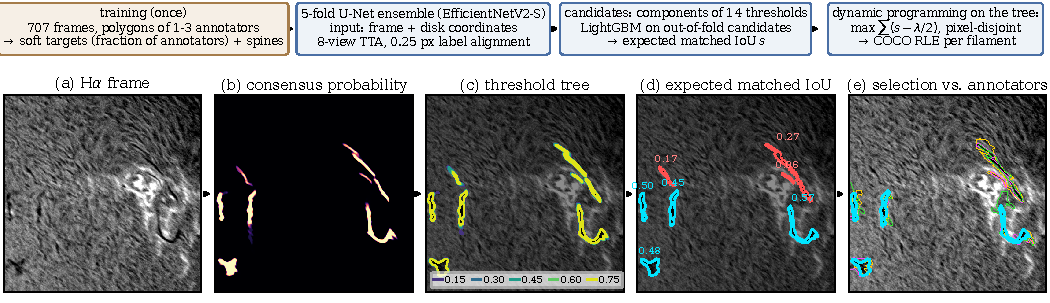
\includegraphics[width=\textwidth]{figures/fig_pipeline.pdf}
    \caption{Data flow (top) and its stages on a held-out frame (bottom). (b) average of the fold networks; (c) components of five of the 14 threshold sets; (d) predicted expected matched IoU of selected (cyan) and rejected (red, dashed) candidates; (e) submitted masks (cyan) and the polygons of the three annotators (yellow, magenta, green). The rejected structure at the top was marked by two of the three annotators with poorly agreeing outlines.}
    \label{fig:pipeline}
\end{figure*}

%%%%%%%%%%%%%%%%%%%%%%%%%%%%%%%%%%%%%%%%
%              METHODOLOGY             %
%%%%%%%%%%%%%%%%%%%%%%%%%%%%%%%%%%%%%%%%
\section{Methodology}\label{sec:methodology}

\subsection{Data and split}
    The training file holds 707 observations with 1{,}154 annotator records (411, 145 and 151 observations with one, two and three independent annotators) and 8{,}199 single-polygon filaments (median area 1{,}228\,px). Polygons are rasterised with pycocotools, i.e.\ exactly like the ground truth of the competition (our pixel areas equal the \texttt{area} field for all annotations). Images are used as provided (8-bit, $2048^2$); the solar disk is centred with a radius of 900\,px in every frame. No other annotations, no file-name metadata and no neighbouring frames are used.
    All experiments use one five-fold split over \emph{observations}: the records of all annotators of an observation share a fold, and every number in Sec.~\ref{sec:evaluation} is computed on observations that neither the network nor the candidate scorer has seen.

\subsection{Consensus probability network}
    \textbf{Targets.} For an observation with $k$ annotators the target of a pixel is the fraction of the $k$ annotators whose polygons cover it. With a cross-entropy loss the network then estimates the probability that a random annotator marks the pixel, instead of imitating a single annotator. The provided \texttt{spine} polylines (drawn 3\,px wide) supervise a second output in the same way; it is only used as evidence by the scorer. Polygons below 30\,px are treated as slips.

    \textbf{Network.} A U-Net \cite{ronneberger2015unet} with an ImageNet-pretrained EfficientNetV2-S encoder \cite{tan2021efficientnetv2} (22\,M parameters; implementation from \cite{iakubovskii2019smp,wightman2019timm}). The input has three channels: the image and the disk-normalised coordinates $(x/R,\,y/R)$ of each pixel. Annotators skip filaments close to the limb, and a network that sees crops cannot otherwise know where on the disk it is. The pretrained stem is reused by giving the image channel the sum of the RGB filters and initialising the coordinate filters with zeros.

    \textbf{Training.} Random $1024^2$ crops are taken from the native frame through a single affine warp (rotation by any angle, isotropic scale in $[0.75,1.33]$, flip; the coordinate channels are warped along). 70\% of the crops are centred near an annotated filament, the rest uniformly on the disk; observations are sampled proportionally to their number of annotator records, as the metric counts them. Photometric augmentation: gamma, contrast and brightness jitter, mild blur and noise. Loss: binary cross-entropy plus soft Dice on the soft targets (spine output weighted 0.5). AdamW \cite{loshchilov2019adamw}, learning rate $3\!\cdot\!10^{-4}$ with warm-up and cosine decay, weight decay $10^{-2}$, batch 8, 8{,}000 iterations, mixed precision, exponential moving average of the weights. One fold trains in 25 minutes on an RTX~5090.

\subsection{Inference}\label{sec:infer}
    Each fold network processes the full $2048^2$ frame in eight views (four rotations, with and without mirroring); the 40 probability maps are averaged.
    The map is then moved up by 0.25\,px. The reason is a systematic offset of the labels: the mean grey level under the annotated polygons is lowest when the polygons are moved \emph{down} by 0.1--0.3\,px (all six annotator groups; no offset in $x$), i.e.\ the polygons sit slightly above the dark filament body. A network trained with rotations and mirrored views cannot represent such an offset, so it is restored afterwards ($+0.002$ PQ; the opposite shift loses the same amount).

\subsection{Candidates, scoring and PQ-optimal selection}\label{sec:select}
    \textbf{What a mask is worth.} PQ \cite{kirillov2019panoptic} pools true positives (pairs with $\mathrm{IoU}>0.5$), false positives and false negatives over all annotator records. Because $|\mathrm{TP}|+|\mathrm{FP}|=N_{\mathrm{pred}}$ and $|\mathrm{TP}|+|\mathrm{FN}|=N_{\mathrm{gt}}$,
    \begin{equation}
        \mathrm{PQ}=\frac{\sum_{(p,g)\in \mathrm{TP}}\mathrm{IoU}(p,g)}{|\mathrm{TP}|+\tfrac12|\mathrm{FP}|+\tfrac12|\mathrm{FN}|}
        =\frac{\sum_{p} m_p}{\tfrac12\,(N_{\mathrm{pred}}+N_{\mathrm{gt}})},
    \end{equation}
    where $m_p$ is the matched IoU of prediction $p$ ($0$ if it has no match). Adding a mask raises the denominator by $\tfrac12$ per record and the numerator by $m_p$; it helps iff its \emph{expected} matched IoU $s_p=\mathbb{E}[m_p]$ exceeds $\mathrm{PQ}/2$. Among alternative segmentations of the same region the best set maximises $\sum_p (s_p-\lambda/2)$ with $\lambda$ equal to the attained PQ \cite{dinkelbach1967fractional}.

    \textbf{Candidates.} The probability map is thresholded at 14 levels ($0.15,0.20,\dots,0.80$). The 8-connected components of all levels form a forest \cite{salembier1998maxtree}: each component lies inside exactly one component of the level below. Every node (holes filled, $\ge 40$\,px, roots $\ge 80$\,px) is a candidate, about 138 per frame. A low-level node is a generous outline or a merged structure, its descendants are tighter outlines or its parts, so the tree contains the alternatives on which annotators disagree.

    \textbf{Scorer.} A LightGBM regressor \cite{ke2017lightgbm} (500 trees, 15 leaves) predicts $s_p$ from 54 descriptors of a candidate: threshold level and position in the tree (area ratios to root, parent and children, number of further levels it survives), statistics of the filament and spine probabilities inside the mask and in two rings around it, image contrast against the rings, shape (principal axes, elongation, perimeter, solidity), position on the disk ($r/R$, $|x|/R$, orientation relative to the radial direction) and frame-level context. The regression target is the mean over the annotator records of $\mathrm{IoU}\cdot[\mathrm{IoU}>0.5]$ with the best-overlapping annotated filament. The scorer is trained on the 97{,}572 out-of-fold candidates of the training observations and cross-fitted with the same folds.

    \textbf{Selection.} With $V(v)$ the best attainable value inside the subtree of node $v$,
    \begin{equation}
        V(v)=\max\Bigl\{\,s_v-\tfrac{\lambda}{2},\ \sum_{c\in\mathrm{children}(v)}V(c),\ 0\Bigr\},
    \end{equation}
    one bottom-up pass yields the optimal pixel-disjoint subset (a node excludes its descendants). We use $\lambda=0.60$: cross-validated PQ is flat for $\lambda\in[0.46,0.60]$ and the larger value compensates for the optimism of selecting on noisy scores. The selected masks are written as COCO run-length encodings. The test set (180 frames) is processed in under eight minutes on one GPU.

\begin{figure*}[t]
    \centering
    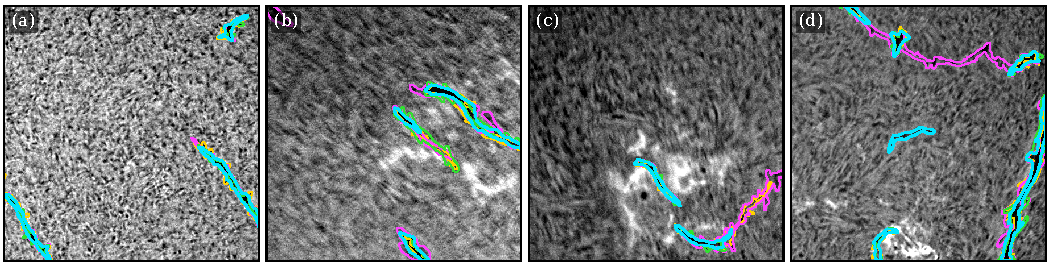
\includegraphics[width=\textwidth]{figures/fig_examples.pdf}
    \caption{Held-out results (cyan) with the polygons of the three annotators (yellow, magenta, green). (a,\,b) thin filaments with barbs; (c) a filament marked by two annotators is not submitted; (d) one annotator draws a single long filament where the others and the model see separate ones, and the model adds a filament nobody marked.}
    \label{fig:examples}
\end{figure*}

%%%%%%%%%%%%%%%%%%%%%%%%%%%%%%%%%%%%%%%%
%              EVALUATION              %
%%%%%%%%%%%%%%%%%%%%%%%%%%%%%%%%%%%%%%%%
\section{Evaluation}\label{sec:evaluation}
    \textbf{Strategy.} All values are out-of-fold over the 707 training observations and use the organisers' definition (each annotator record is compared with the predictions of its image; counts are pooled). Our implementation returns the same PQ as the functions of the public self-evaluation notebook on a written and re-read submission file. Uncertainty is given as the standard deviation of 1{,}000 bootstrap resamples of observations and as the spread over folds.

    \textbf{Results.} Table~\ref{tab:results} compares the stages. Selecting masks by expected matched IoU adds 0.020 PQ to tuned thresholding, almost entirely through recognition quality: outlines are already as good as annotators allow (the mean IoU of matched pairs is 0.68, Dice 0.81, against 0.63 between annotators). The folds give 0.479, 0.458, 0.453, 0.459 and 0.447 (s.d.\ 0.012), which is the spread expected from random sets of 141 observations (0.009), so no fold behaves differently. PQ is 0.455, 0.471 and 0.457 on observations with one, two and three annotators. With true scores the same candidates would reach 0.559; the remaining gap is the unpredictable part of the annotators' choices.
    For the relations between ground truth and prediction: 74.5\% of the annotated filaments overlap exactly one predicted mask, 3.1\% overlap several (fragmentation) and 22.4\% none; 87.2\% of the predicted masks overlap exactly one filament of a record, 2.4\% several (merging) and 10.4\% none.
    The model agrees with an annotator more often than a second annotator does, at every size (Fig.~\ref{fig:eval}). On the public leaderboard the five-fold ensemble scores 0.40, a single fold network 0.38, and the same network with plain thresholding 0.36.

\begin{table}[t]
    \caption{Out-of-fold results on the 707 training observations (1{,}154 annotator records).}
    \label{tab:results}
    \small
    \begin{tabular}{@{}lccc@{}}
        \toprule
        & PQ & SQ & RQ \\
        \midrule
        another annotator of the same image & 0.340 & 0.634 & 0.536 \\
        threshold 0.45, components $\ge 400$\,px & 0.435 & 0.682 & 0.638 \\
        \quad + hysteresis (0.45/0.15), tuned & 0.440 & 0.682 & 0.645 \\
        tree + scorer + selection (submitted) & \textbf{0.460}\,$\pm$\,0.004 & 0.685 & 0.672 \\
        \midrule
        same candidates, true scores (bound) & 0.559 & -- & -- \\
        \bottomrule
    \end{tabular}
\end{table}

\begin{figure}[t]
    \centering
    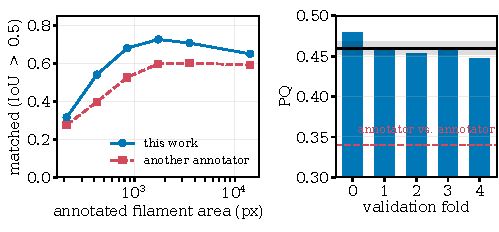
\includegraphics[width=\columnwidth]{figures/fig_eval.pdf}
    \caption{Left: share of an annotator's filaments matched at $\mathrm{IoU}>0.5$ by the model and by another annotator (observations with several annotators). Right: PQ per validation fold; line and band: pooled value and its 95\% bootstrap interval.}
    \label{fig:eval}
\end{figure}

    \textbf{What did not help.} Table~\ref{tab:ablation} lists the variations we tested. Their common message is that the network and the candidates are not the bottleneck: architectures, loss, schedule and ensembling move PQ by less than the fold noise, and every attempt to edit the masks or to add candidates failed.

\begin{table}[t]
    \caption{Variations of the pipeline ($\Delta$PQ against the submitted configuration; f0 = validation fold 0 only).}
    \label{tab:ablation}
    \small
    \begin{tabular}{@{}lr@{}}
        \toprule
        variation & $\Delta$PQ \\
        \midrule
        8-view instead of 4-view test-time augmentation (f0) & $+0.003$ \\
        label alignment by $-0.25$\,px / by $+0.25$\,px (3 folds) & $+0.002$ / $-0.002$ \\
        average of two encoder families (f0) & $+0.002$ \\
        cross-entropy without Dice (f0) & $-0.001$ \\
        RegNetY-040 / ConvNeXt-T encoder (f0) & $-0.006$ / $-0.004$ \\
        2.5$\times$ longer schedule, stopped half-way (f0) & no gain \\
        7 / 31 threshold levels instead of 14 & $0.000$ / $-0.003$ \\
        fragments grouped or split along spines as candidates & $0.000$ \\
        masks dilated / eroded by one pixel (f0) & $-0.016$ / $-0.037$ \\
        second-stage mask refiner per candidate (f0) & $-0.004$ \\
        CNN view of the candidate as extra descriptor (3 folds) & $-0.002$ \\
        \bottomrule
    \end{tabular}
\end{table}

    \textbf{Strengths.} The selection step is derived from the metric and exact, has one interpretable parameter, and replaces hand-tuned thresholds, minimum areas and merging rules. The whole system is one network architecture plus a small tabular model; it trains in two GPU-hours and is validated without leakage.
    \textbf{Weaknesses.} (1)~Performance is bounded by annotator disagreement, not by image evidence: 22\% of the annotated filaments receive no mask because marking them is not predictable from the image (27\% of the filaments below 300\,px are matched against 70\% between 1{,}200 and 5{,}000\,px), and 14.5\% are overlapped but fail the IoU threshold, mostly where annotators differ on whether pieces form one filament (Fig.~\ref{fig:examples}d). (2)~Close to the limb ($r/R>0.9$) hardly anything is matched. (3)~Level sets of a consensus map smooth out barbs that only some annotators draw.
    \textbf{Possible improvements.} Consensus labels for the observations that have a single annotator would raise the ceiling for every method; an explicit model of the annotator could separate style from image content; and information that is physically relevant for filament identity (magnetograms, the evolution over neighbouring frames) could resolve grouping ambiguities that a single frame cannot.

    \textbf{Disclosure.} Only the competition training file and an ImageNet-pretrained encoder were used; the public MAGFiLO release was never used. An AI coding assistant was used to implement and run the experiments.

%%%%%%%%%%%%%%%%%%%%%%%%%%%%%%%%%%%%%%%%
%            ACKNOWLEDGMENT            %
%%%%%%%%%%%%%%%%%%%%%%%%%%%%%%%%%%%%%%%%
\section{Acknowledgment}\label{sec:acknowledgment}
    % Do not change
    The organization of the Filament Segmentation Challenge 2026 is partially supported by the U.S. National Science Foundation (NSF) under Grant No. 2209912 and 2433781, directorate for Computer and Information Science and Engineering (CSE), and Office of Advanced Cyberinfrastructure (OAC), and Grant No. 2511630, AST Division Of Astronomical Sciences and MPS Directorate for Mathematical and Physical Sciences.

    The Filament Segmentation Challenge 2026 is sponsored by the U.S. National Science Foundation (NSF) National Solar Observatory (NSO).

    This work utilizes GONG data obtained by the NSO Integrated Synoptic Program, managed by the National Solar Observatory, which is operated by the Association of Universities for Research in Astronomy (AURA), Inc. under a cooperative agreement with the National Science Foundation and with contribution from the National Oceanic and Atmospheric Administration. The GONG network of instruments is hosted by the Big Bear Solar Observatory, High Altitude Observatory, Learmonth Solar Observatory, Udaipur Solar Observatory, Instituto de Astrofísica de Canarias, and Cerro Tololo Interamerican Observatory.

\bibliographystyle{ACM-Reference-Format}
\bibliography{main}

\end{document}
